\section{Численные методы решения}
\label{sec:algrhtms}

Далее мы опишем алгоритмы использующиеся для решений уравнений
эйконала. Это два разных метода, базирующиеся на разных и идеях и,
следовательно, пригодные для разных целей. Один заточен для
максимального ускорения работы и, как это часто бывает с такими
алгоритмами практически неспособен к параллелизации, другой же --
наоборот работает несколько медленнее, но гораздо проще поддается
распараллеливанию.

\subsection{Общая идея методов}
\label{sec:general-idea}

Для всех методов нам необходимо научится решать задачу в локальном
случае. Разберем для начала одномерный случай. Пусть нам дано
следующее уравнение эйконала:

\begin{equation}
  \label{eq:eik_smp}
  \sqrt{(\frac{dT}{dx})^2}=F(x), T(-1) = T(1) = 0.
\end{equation}

% Вставить куда-нибудь ссылку
Для упрощения обозначений мы запишем производную $T$ по $x$ в виде
$T_x$. Также в будущем мы будем поступать и для частных
производных. После преобразования уравнение~\eqref{eq:eik_smp} примет вид:

\begin{equation*}
  \sqrt{T_x^2}=F(x), T(-1) = T(1) = 0.
\end{equation*}


Имеется функция скорости $F(x) > 0$, требуется построить
решение $T(x)$. Мы видим, что решение не уникально (если t(x) решает
задачу, то тогда и $-t(x)$ также ее решает). Будем работать только с
положительными решениями.

Рассмотрим обыкновенное дифференциальное уравнение и разобьем решение
на подзадачи:

\begin{equation*}
  \left\{
      \begin{array}{ll}
        T_x = ~F(x), \quad x \ge 0,\\
        T_x = -F(x), \quad x \le 0,\\[0.3cm]
        T(-1)= T(1) = 0.
      \end{array}
    \right.
\end{equation*}

Для численной аппроксимации разобьем ось $x$ на набор точек сетки
$x_i=i\Delta x$. Положим $T_i = T(i \Delta x)$ и $F_i = F(i \Delta
x)$, где $\Delta x$ - это шаг дискретизации, $i = -n, \cdots,
n$. Далее используем разложение Тейлора и отбросим остаток. Получим
следующую дискретную систему:

\begin{equation}
  \label{eq:discretise}
  \left\{
    \begin{array}{ll}
      T_n = 0,\\
      \frac{T_{i+1} - T_i}{\Delta x} = F_i, \quad i>0 \\\
      \frac{T_{i} - T_{i-1}}{\Delta x} = F_i, \quad i>0\\
      T(-n) = 0\\
    \end{array}
  \right.
\end{equation}

Отметим, что
\begin{itemize}
\item[ ] $T_{n-1}$ может быть получено из $T_n$
\item[ ] $T_{n-2}$ может быть получено из $T_{n-1}$
\item[ ]  $\cdots$
\item[ ] $T_{1}$ может быть получено из $T_2$
\item[ ] $T_{0}$ может быть получено из $T_{1}$
\item[ ]  $\cdots$
\item[ ] $T_{-n+1}$ может быть получено из $T_{-n}$
\item[ ] $T_{-n+2}$ может быть получено из $T_{-n+1}$
\item[ ]  $\cdots$
\item[ ] $T_{-1}$ может быть получено из $T_{-2}$
\item[ ] $T_{0}$ может быть получено из $T_{-1}$

\end{itemize}

Выше мы построили разностную схему, где вычисляем производные двигаясь
по направлению распространения границы: каждое следующее уравнения вне
текущей границы получено на основании уже имеющихся решений внутри
нее.

Вычисляя уравнение эйконала мы видим, что информация распространяется
как волны с определенной скоростью вдоль направления градиента. Наш
метод дискретизации вычисляет значения переменных используя
направления того откуда информация о решениях приходит. Если говорить
точнее, то дискретизация уравнений в частных производных использует
конечно-разностную трассировку смещающуюся в направлении знака
градиента.

Для одномерного случая у нас есть только два направления для каждой
точки $i$: правое $(i+1)$ и левое $(i - 1)$. Предположим, что у нас
есть решение в точке $i$, на итерации с номером $n$. Тогда мы имеем
два случая:
\begin{itemize}
\item Правое направление: $T_i^{n+1} = T_i^n - \Delta x D^{+x}_iT(x_i)$
\item Левое направление: $T_i^{n+1} = T_i^n - \Delta x D^{-x}_iT(x_i)$
\end{itemize}

Здесь мы приняли следующие обозначения из \eqref{eq:discretise}:

\begin{equation*}
  \begin{array}{ll}
    & D^{+x}_iT(x_i) = \frac{T_{i+1} - T_{i}}{\Delta x} \\
    & D^{-x}_iT(x_i) = \frac{T_{i} - T_{i-1}}{\Delta x}
  \end{array}
\end{equation*}

Подобным образом используя разложение Тейлора в $x1$ и $x2$ для
величины $T$ мы можем определить эти обозначения для двумерного
случая, задав тем самым регулярную двумерную сетку дискретизации,
тогда для точек $(x1,x2)$, с разбиением
$(x1_i,x2_i) = (i\Delta x,j \Delta y)$ и $T_{ij} = T(x1_i,x2_i)$ мы
получим:

\begin{equation}
  \label{eq:discrete-defines}
  \begin{array}{ll}
    D^{-x1}_{i,j}T(x1,x2) = \frac{T_{i,j} - T_{i-1,j}}{\Delta x1}  \\
    D^{+x1}_{i,j}T(x1,x2) = \frac{T_{i+1,j} - T_{i,j}}{\Delta x1}  \\
    D^{-x2}_{i,j}T(x1,x2) = \frac{T_{i,j} - T_{i,j-1}}{\Delta x2}  \\
    D^{+x2}_{i,j}T(x1,x2) = \frac{T_{i,j} - T_{i,j+1}}{\Delta x2}  \\
  \end{array}
\end{equation}

\begin{itemize}
\item $D^{+x1}$ вычисляет новое значение в узле сетки $(i,j)$ используя
  информацию из $i$ и $i+1$, таким образом информация для решения
  распространяется справа налево.

\item $D^{-x1}$ вычисляет новое значение в узле сетки $(i,j)$ используя
  информацию из $i$ и $i-1$, таким образом информация для решения
  распространяется слева направо.
\item $D^{+x2}$ вычисляет новое значение в узле сетки $(i,j)$ используя
  информацию из $j$ и $j+1$, таким образом информация для решения
  распространяется сверху вниз.

\item $D^{-x2}$ вычисляет новое значение в узле сетки $(i,j)$ используя
  информацию из $j$ и $j-1$, таким образом информация для решения
  распространяется снизу вверх.

\end{itemize}

Для двумерного случая разностные схемы действуют вдоль направления
градиента. На рисунке~\ref{fig:upwind-schema} иллюстрируются две
возможных ситуации. В первом случае распространение информации идет из
третьего квадранта, В другом случае -- из второго


\begin{figure}[h]
  \centering
  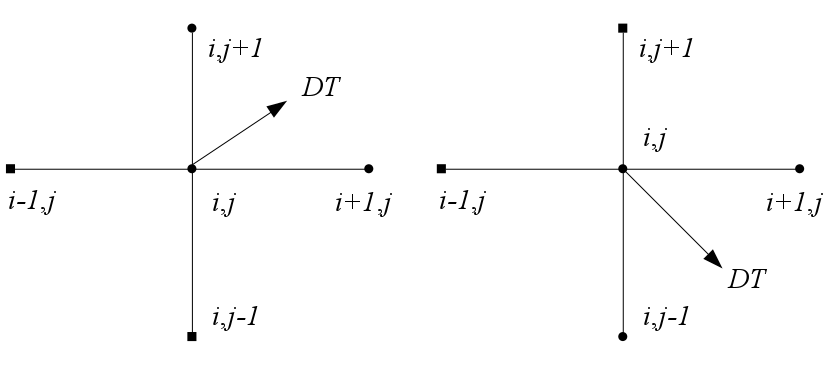
\includegraphics[width=\linewidth]{img/upwind-schema.png}
  \hfil \caption{Пример разных направлений распространения}
  \label{fig:upwind-schema}

\end{figure}

Крэндалл и Лайонс в \cite{V1983} доказали, что последовательные
монотонные схемы сходятся к корректному вязкостному решению.

\subsection{Fast sweeping method}
\label{sec:fast-sweeping-method}

Fast sweeping method (метод быстрых выметаний. обычно даже в
русских публикациях не переводится) далее FSM -- итеративный метод, который
использует разностную схему для дискретизации уравнения эйконала
\cite{F2005}. Идея, скрывающаяся за FSM это ``замести'' сетку в
определенных направлениях. Порядок выметания определяется
характеристиками соответствующего уравнения эйконала

\subsection{Fast marching method}
\label{sec:fast-marching-method}


\subsection{Нерегулярная сетка}
\label{sec:unstructured-mesh}

\subsubsection{Триангуляция}
\label{sec:triangulate}

\subsection{Вопросы реализации}
\label{sec:programming}



%%% Local Variables:
%%% mode: latex
%%% TeX-master: "eikonal_solver"
%%% End:
